% \chapter{Data Preprocessing}
\chapter[BranMorph: a morphological tool for TGCs]{BranMorph: extracting morphological features and classifying}
\label{chap: branMorph}
% \label{chap:preproc}

\section{A proposal for \emph{tip-growing cells} morphometry}

As we can see, the whole cell morphology in almost all \acfp{TGC} share some common features and could be fit into a kind of model based on branches and skeletons. By modeling a neuron into a tree-like shape or graph, research on neuron morphology has accumulated lots of such reconstructions as shown in the database NeuroMorpho.Org, and software packages as mentioned in chapter \ref{chap: introMorph}. BranMorph ports the idea to other \acfp{TGC}, especially pollen tubes, the research on which to date lacks dedicated computational analysis tools, and extends the idea into collection of features based on the skeleton-like representations as in neuron morphology.

To give a first impression, branMorph is proposed to be distinguished by these features:

\begin{itemize}
\item \textbf{\ac{ISAT}}. Seeing the variablity in both image quality and \emph{tip-growth cell} morphology, global segmentation methods alone are too weak to achieve reliable fully automated processing, whereas the \ac{ISAT} complements the power of segmentation algorithms by human interaction to make accurate results while minimizing human interaction and making interaction comfortable and convenient.
\item \emph{Quantitative cell morphology comparison and presentation}. The conventional approach to report cell morphology is by displaying one or two typical cell images to give a qualitative and intuitive comparison. Nevertheless, transforming the morphology images quantitatively and presenting the whole dataset with its distribution plotted, for example in 2D or 3D \ac{PCA} plots, would doubtlessly make the result more convincing.
\item A model theoretically able to cover almost all relevant morphological features for \acp{TGC}.
% \item It's based on the image skeletonization algorithms.
% \item It's basic output is a data structure named as \emph{woods}. \emph{Woods} borrows the ideas from the notion of tree structure and forest sturcture. Forest structure consists lots of trees. \emph{woods} structure consists less but several trees.
% \item Seeing that the preprocessing is vital to the whole manipulation, \emph{branMorph} provides several useful interactive utility functions to aid the preprocessing.
\end{itemize}

% In this report, we propose an automatic measure method based on the image morphological processing. With the proposed method, high-through put image processing is on the way to be feasible.

\section{Sample Preparation and Image Acquisition}
\label{sec: data}

% \subsection{Neuron images}

The data used in classification are mainly pollen tube images. One neuron image is used for demonstration in previous chapters (kindly provided by Dr. Zhi Yang from Institute of Neuroscience) was taken from a set of \emph{in vitro} growth experiments of neurons. The neuron image is for demonstrating the ability of \emph{branMorph} to processing neuron images and quantifying morphological features from them, so the acquisition detail of such an image is omitted here.

% \todo{More on this data? what sample, what labels, what microscope? Or just skip this subsec?}

% \todo{Use this data?} Another image set denoted here as CIL8787 is downloaded from The \href{http://www.cellimagelibrary.org/images/8787}{Cell: An Image Library™}. The image set shows the co-localization of filamentous actin (red) and microtubule array (green) in a bundle of cultured embryonic rat hippocampal neurons, and its attribution goes to Dieter Brandner and Ginger Withers.

\subsection{Simulated pollen tube images}

Because some morphology, e.g. swollen-in-middle, is rarely found in our real data, we manually produced artificial pollen tube images in 6 groups same as the groups in morphologically distinguished data in section \ref{subsec: morphGroup}: \emph{balloon}, \emph{wavy}, \emph{branch}, \emph{swollen}, \emph{thin} and \emph{wildtype}. These simulated data is used to demonstrate the classification power of the skeleton-based features. Besides, the simulated data is also included in the software package of \emph{branMorph} as \emph{simuPollens}, in order to provide easy-to-get-on examples for fresh users to practise.

All simulated images are 500 pixels by 500 pixels in RGB mode since the software \emph{branMorph} does not accept binary or grayscale images. The simulation parameters could be infered from the filenames, for example, the image called branch2\_gd63\_tw21\_tr24.png belongs to \emph{branch} group and has 2 branches, its pollen grain diamter is 63 pixels, tube width 21 pixels and tip diameter is 24 pixels.

\begin{table}
\caption[Parameters of simuPollens]{\emph{Parameters used in simulated pollen images}. The acronyms for each parameter are given in parentheses behind the parameter. Except branch number and wavy number, the range of all other parameters are given in pixels.}
{\scriptsize \tt
\begin{tabular}{ccccccc}
\toprule
\backslashbox{Parameters}{Groups} & Branch & Swollen & Wildtype & Balloon & Thin & Wavy \\\midrule
Branch number & $2\sim~3$ & 0 & 0 & 0 & 0 & 0 \\\midrule
Grain diameter (gd) & $60\sim~65$ & $50\sim~62$ & $48\sim~62$ & $50\sim~60$ & $47\sim~52$ & $48\sim~60$ \\\midrule
Tube width (tw) & $20\sim~25$ & $23\sim~30$ & $19\sim~32$ & $23\sim~33$ & $10\sim~13$ & $20\sim~30$ \\\midrule
Tip diameter (tr) & $24\sim~55$ & $25\sim~30$ & $23\sim~34$ & $70\sim~90$ & $14\sim~16$ & $22\sim~33$ \\\midrule
Middle bubble diameter (mr) & 0 & $48\sim~70$ & 0 & 0 & 0 & 0 \\\midrule
Wavy number (wavy) & 0 & 0 & 0 & 0 & 0 & $6\sim~10$ \\\bottomrule
\end{tabular}
}
\end{table}

\subsection{Pollen tube images}

Different gene constructs were transferred by colloidal gold bombardment method and transiently over-expressed \parencite{Twell1989transient}.

%	The genes are transfered by colloidal gold method.
%  The CCD camera scale used in pollen tube images may be 20X.

% \begin{itemize}
% \item W32: Pollen tube expressing GFP only is normal.
% \item W42: Overexpressing LePRK1-eGFP increased the pollen tube width and caused ballooned tips with bubble-like entities.
% \item G16: Overexpressing KPP-eGFP moderately increased the pollen tube width.
% \item G145 and G16: Coexpressing G16 and a gene we numbered G145 also caused ballooned tips with bubble-like entities, though with a low frequency.
% \end{itemize}

Images were captured using an Olympus BX51 microscope fitted with an Olympus DP71 digital camera after 4-6 hours cultivation.

All experiments were conducted with tobacco pollens, where the radius of pollen grain was about 15\,$\mu$m. The scales used on the object lense are 20$\times$ and 40$\times$. In our method, we first calculated the lengths in pixels and afterwards re-scale the lengths to a 20$\times$ level, i.e., divided all lengths from 40$\times$ images by 2, so that all the lengths or areas output are comparable. For the same reason, the areas from 40$\times$ images are divided by 4. In abstraction of Murphy features, 20$\times$ scaled images used 0.2131\,$\mu$m per pixel as the \emph{scale} input, and 40$\times$ used 0.1065\,$\mu$m per pixel.

\section{Cropping}

Microscopic images obtained often display several individual cells, usually only one of which is considered the cell of interest. Selecting this cell of interest is achieved by a semi-automated cropping procedure. The program thresholds the original image using Otsu's method \cite{Otsu:1975}, fills holes, finds the largest connected component and calculates the minimal rectangle holding the largest connected component with some paddings. The user may manually adjust the rectangle either in position and size, and confirm after the result is satisfactory.

Cropping could also be applied to split a big image containing two or more cells of interest into several smaller images. Another benefit of it is reducing the background pixels and thereafter boosting processing speed. See \figRef{fig: cropping}.

\begin{figure}
\caption[Interactive Cropping]{\label{fig: cropping} \emph{Interactive Cropping}. (a) shows the initial cropping frame calculated by first global thresholding, finding the largest connected component and then setting the frame with some extra paddings. (b) is the manual adjustment result, where the cropped image is reduced almost by a half in size.}
\subfloat[Initial frame by global thresholding]{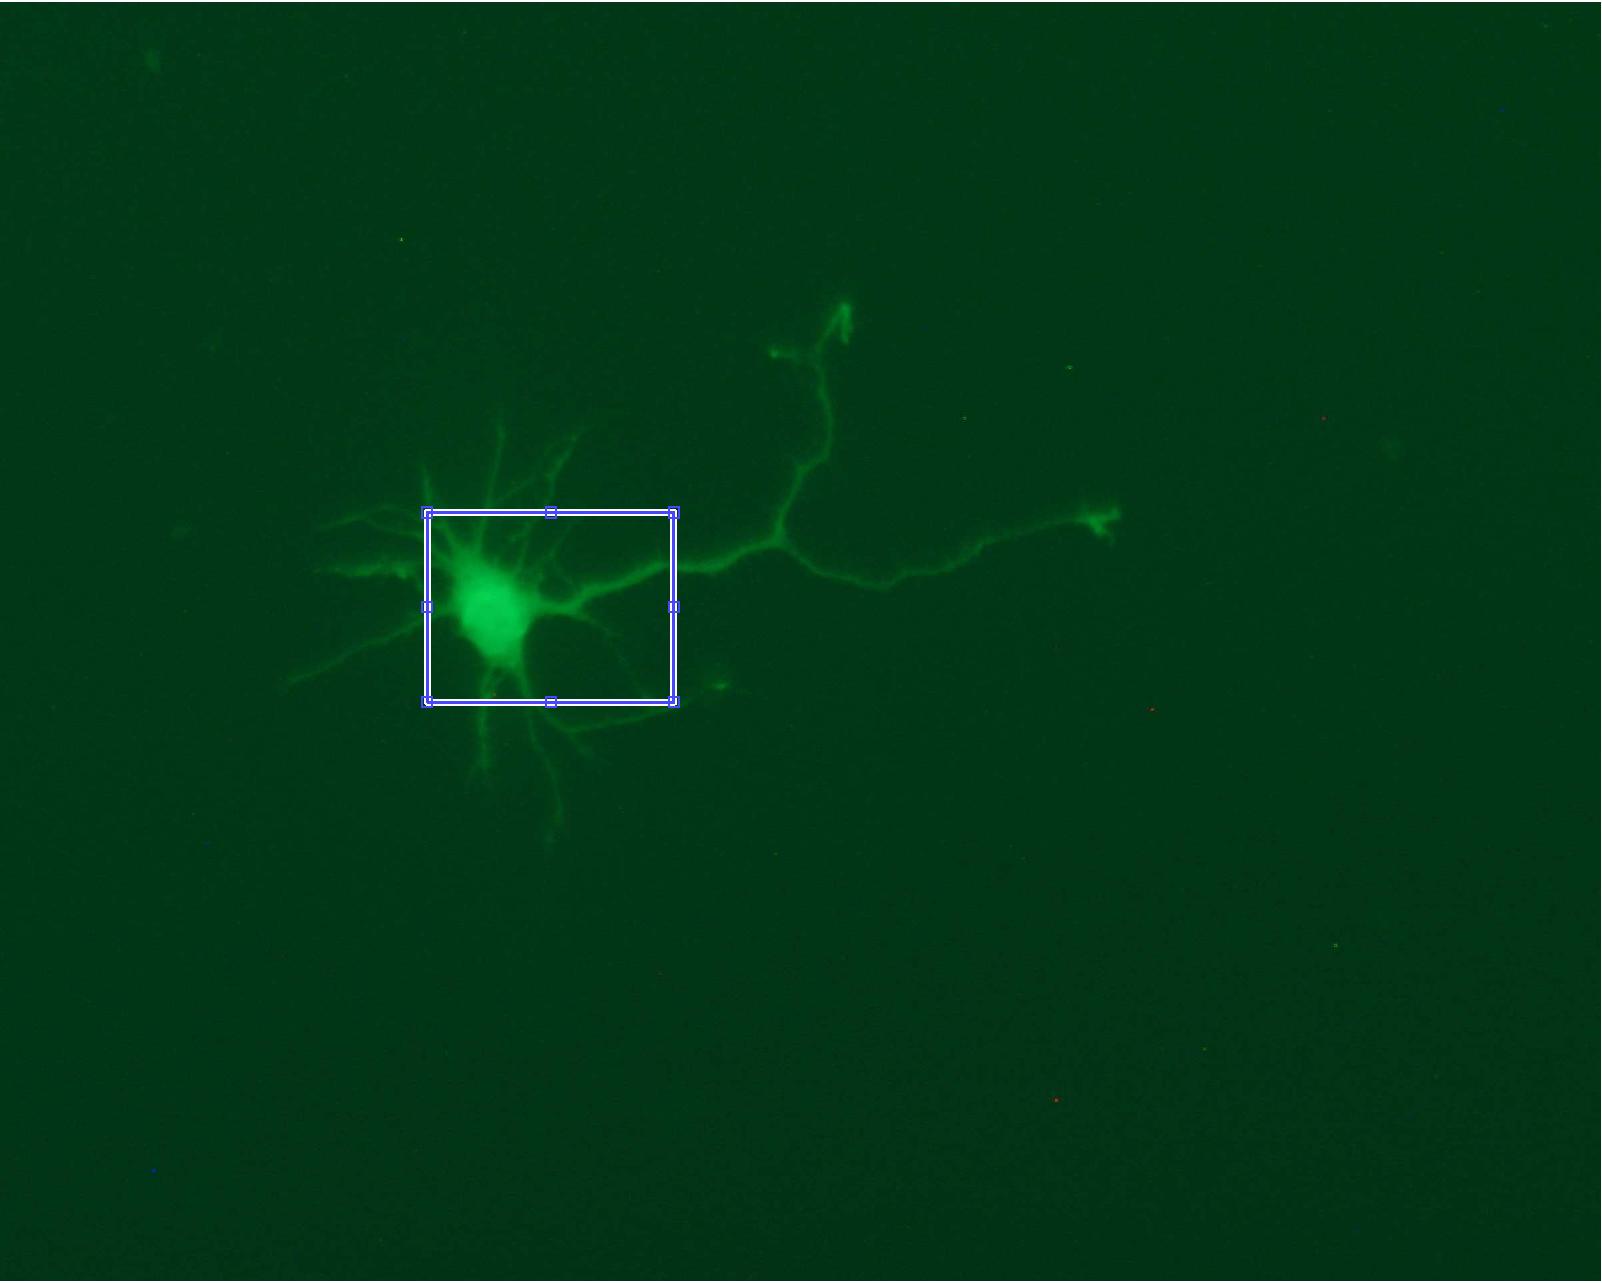
\includegraphics[width=0.4999\textwidth]{crop1.pdf}}
\subfloat[After manual adjustment]{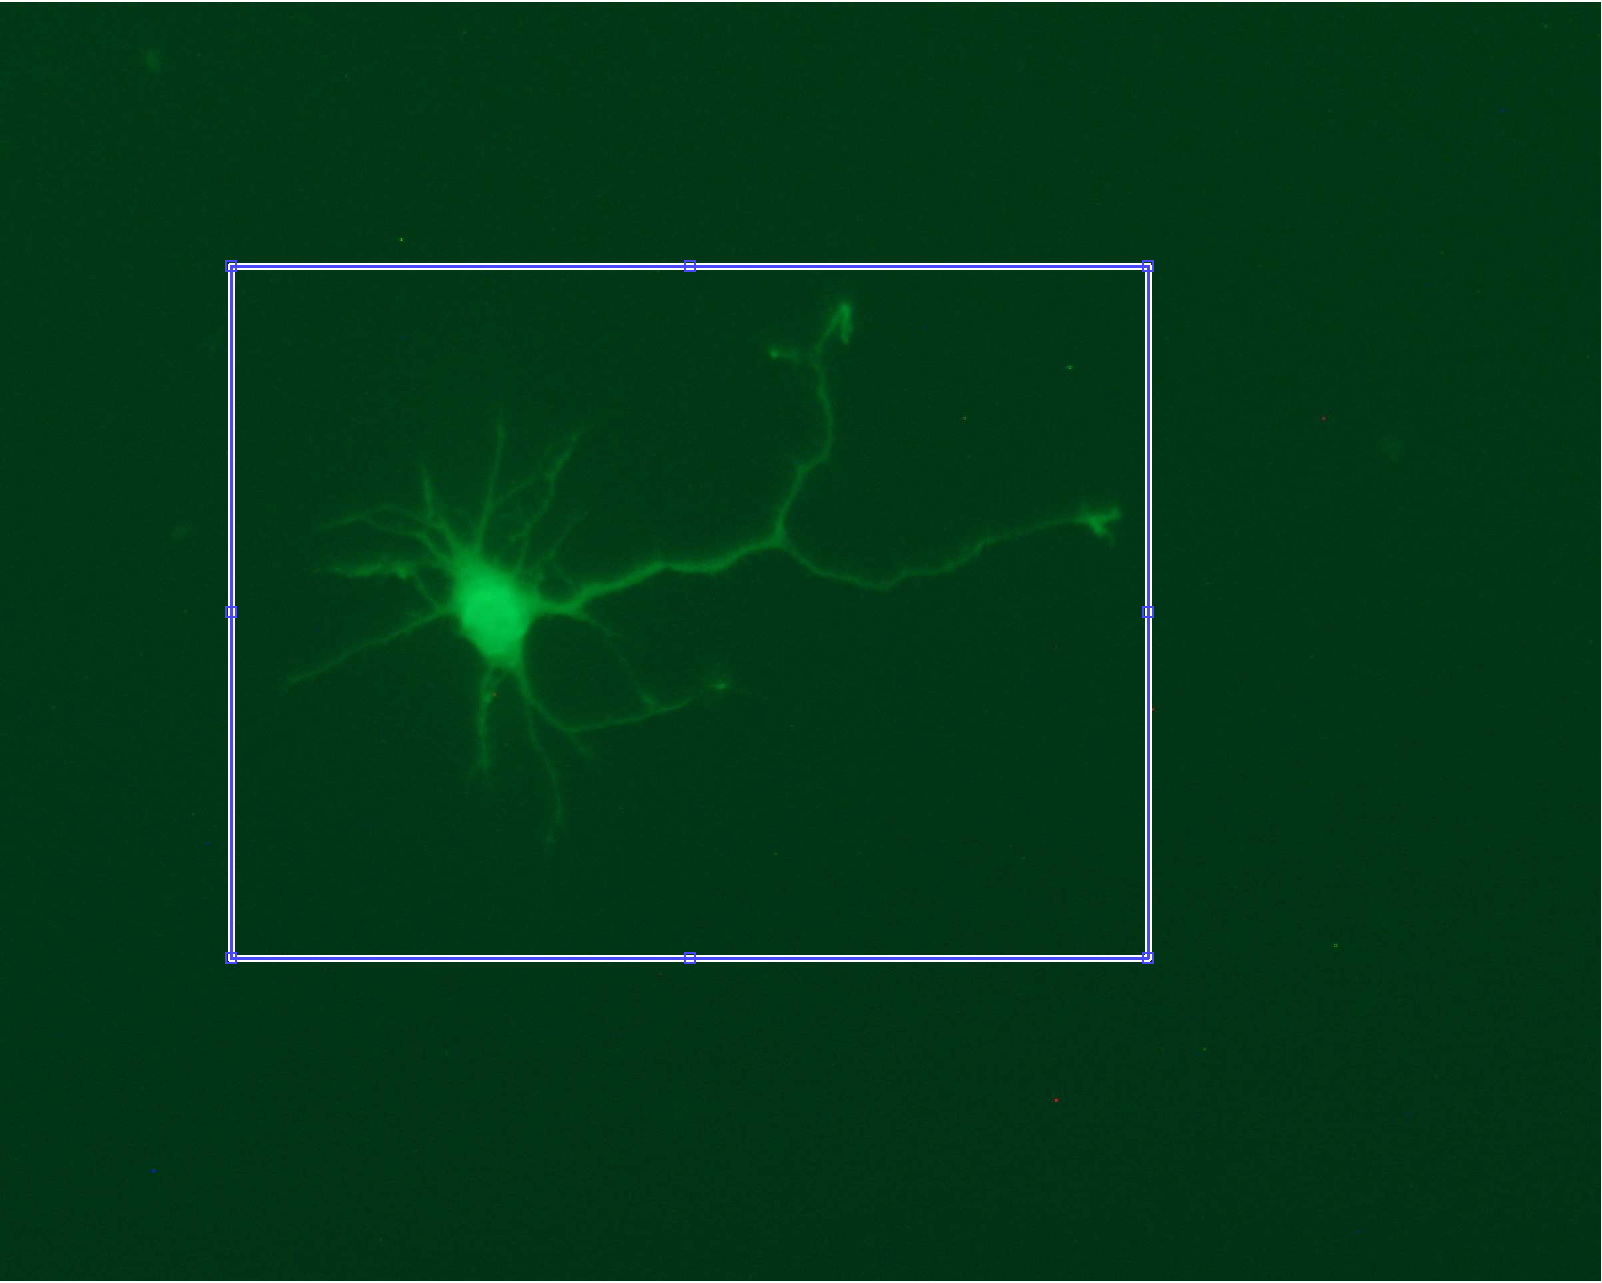
\includegraphics[width=0.4999\textwidth]{crop2.pdf}}
\end{figure}

% TODO:
% Neuroml examples: http://www.neuroml.org/NeuroMLValidator/Samples.jsp

% \todo{Use NeuronJ to make manual annotation}

% \todo{Use neuronConstruct to procude some simulated neuron morph data for testing.}

% NLMorphologyViewer could be used to view swc, neuronml .etc files.

\section{Semi-automated cell segmentation}

Obtaining a proper segmentation is essentially important to feature abstraction. Automatically or manually global thresholding, and image enhancement are usually implemented for such sake. However, from a general perspective, images with debris or non-interesting cells, complicated by uneven illumination, cause global thresholding to fail. Image enhancements such as histogram adjustment and local adaptive thresholding are only applicable to a specific type of images, since using the same parameters of these methods to process a different dataset could be errorneous. Thus we devised a semi-automated image segmentation tool, which requires only simple mouse operations from an investigator and performs a segmentation for a cell in a minute. (Both the semi-automated image segmentation tool and the skeleton feature extraction codes are writen and run in Matlab environment. The codes are availble on \url{http://github.com/silencej/pollenTubeProc} under GPLv3 licence.)

% \subsection{Segmentation}

Based on the cropped region of a cell of interest, a correct segmentation separating the region belonging to the pollen from background is required, and as \figRef{fig: ISATComp} shown, inaccuracy in segmentation may cause a wrong skeleton structure. Due to the speckle noises, weak fluorescence intensity and highly inhomogeneous distribution of fluorescence inside the pollen, this is generally not possible using a global threshold. We thus stretch the image histogram, eliminate speckle noises, and adopt a semi-automated method to fulfill the segmentation.

% \todo{a flow chart for the segmentation process.}

% The process comprised the following phases: \ldots.

\subsubsection{Notational conventions}

For convenience, we introduce the notational conventions as follows. We write $[a:b]$ for the integer interval $\{a,a+1,\dots,b-1,b\}$, and consider a fluorescence image $I$ as a mapping $I\colon [1:M]\times[1:N]\to[0:Q-1]$, where $M$ and $N$ denote width and height of an image and $Q$ the intensity range. For $A\subseteq[1:M]\times[1:N]$, we denote $I(A)$ for $I$ restricted to the positions in $A$. We use $I\ge\theta$ to denote the set of positions $\{a\in[1:M]\times[1:N]\colon I(a)\ge\theta\}$.

\subsection{Image de-noising and enhancement}

The speckle noises are dealt with by Lee filter as in page \pageref{subsubsec: speckle} with a window size of 9. \ac{CLAHE} is deployed here to enhance the low intensity images especially for neuron images (so we use a neuron image here for demonstration), and we use the tool provided by Matlab Image Processing Toolbox with all parameters set by default. The order of executing Lee filter and CLAHE does not affect results (data not shown).
% For the order of Lee and CLAHE, the testSpekle.m has a cell script producing leeClahe.eps and claheLee.eps.

% See \figRef{fig: claheLee}.

% \begin{figure}[hp]
% \caption[CLAHE and De-speckling]{\label{fig: claheLee} \emph{CLAHE and De-speckling with Lee filter}.}
% \subfloat[Original neuron image in psedocolor.]{\includegraphics[width=0.49\textwidth]{oriImgsc.pdf}}
% \subfloat[Neuron image after CLAHE.]{\includegraphics[width=0.49\textwidth]{oriClaheImgsc.pdf}}\\
% \subfloat[Neuron image after Lee plus CLAHE.]{\includegraphics[width=0.49\textwidth]{leeClaheImgsc.pdf}}
% \end{figure}

\subsection{\acf{ISAT}}

There are often cases that automatic algorithms fail to segment a bunch of images and manual curation should be involved in. The \acf{ISAT} provided by us could easily facilitate the human intervention in an aim of suppressing subjectivity and tediousness in this process to an extent as possile as it can.

This semiautomated approach starting with setting a global threshold obtained from Ostu's method inside the well-cropped region. The user can try to adjust this threshold interactively to obtain a first refined segmentation $S$. After the global threshold is set and the result is presented, the user can interactively identify \emph{refinement regions} (RRs) to correct the existing segmentation. The refinement regions can be defined very coarsely a polygonal line encircling the refinement region that we denote by $R\subseteq[1:M]\times[1:N]$. The RRs can now be used to either extend or reduce the existing segmentation. Using the existing segmentation $S$ and the RR $R$, we can compute the extension area $S_a$ as follows:

$$S_e=(R\setminus (R\cap S))>T_o$$

where $T_o$ is the Ostu-threshold for the region $R\setminus(R\cap S)$. Now, the current segmentation $S$ is refined to $S:=S\cup S_e$.

Reducing $S$ by the RR $R$ works correspondingly. The RR should overlap with the current segmentation and cover the segment to be deleted. The area $S_r$ to be deleted is calculated as

$$ S_r=(R\cap S)<T_o,$$

and the current segmentation is set to $S:=S\setminus S_r$. The refinements based on RRs may introduce sharp edges which are problematic for further analysis, in particular skeletonization. To avoid this, $S_e$ and $S_r$ are subjected to morphological smoothing using image opening followed by image closing.

\begin{figure}
\caption[Intelligent adjustment on user input Region of Interest]{\label{Figure: maskDemo} \emph{Intelligent adjustment on user input Region of Interest.} We could see from \protect\subref{mask-a} that after global thresholding, there are incorrect segmentations emphasized in white box, the right one including unwanted part and the the left one missing the branch. The user input Refinement Regions (\emph{RR}s) as in \protect\subref{mask-b} and \protect\subref{mask-d}, and chose \emph{addition} in \protect\subref{mask-b} and \emph{deletion} in \protect\subref{mask-d}. The results are shown in \protect\subref{mask-c} and \protect\subref{mask-e}. The pollen tube image is in a gray image displayed in pseudo-color, and \protect\subref{mask-a} is rotated by 90 degrees.}
\subfloat[\label{mask-a} After global thresholding]{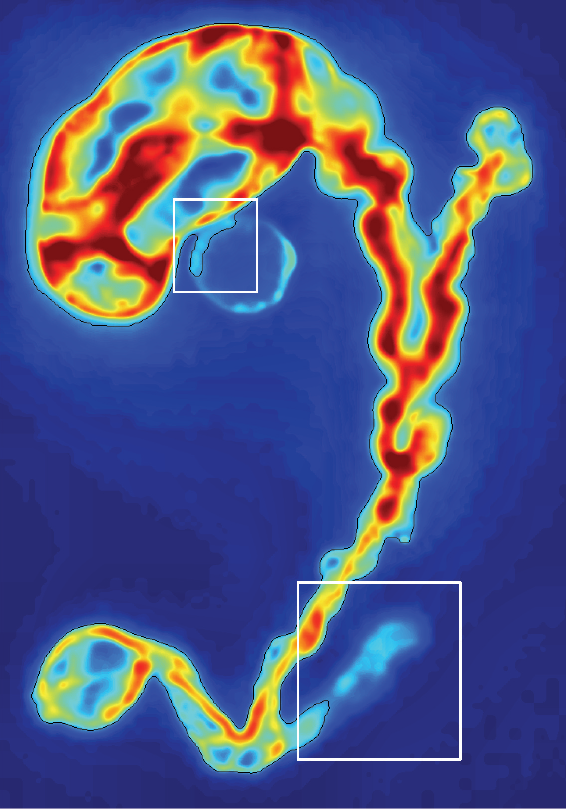
\includegraphics[angle=270,width=0.99\textwidth]{mask-a.pdf}}\\
\subfloat[\label{mask-b} Manually Add]{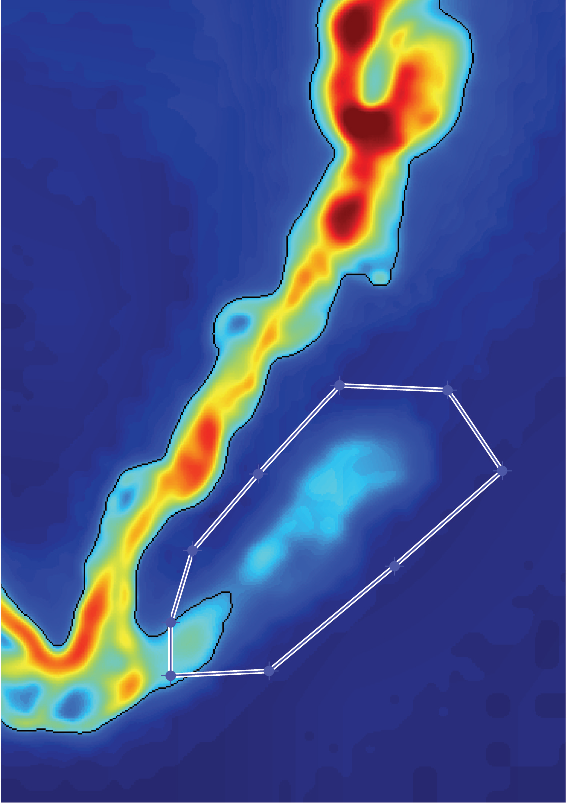
\includegraphics[width=0.249\textwidth]{mask-b.pdf}}
\subfloat[\label{mask-c} Result of addition]{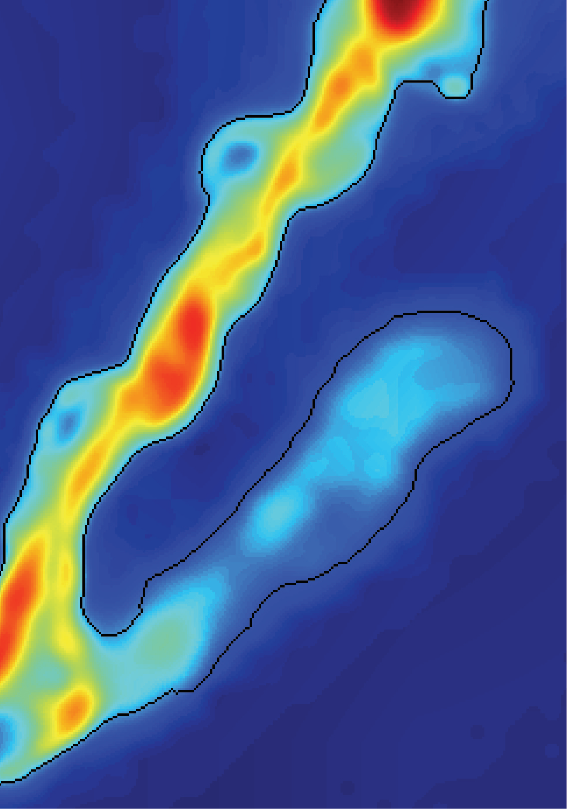
\includegraphics[width=0.249\textwidth]{mask-c.pdf}}
%\subfloat[Part to be deleted]{\includegraphics[width=0.3\textwidth]{mask-d.pdf}}
\subfloat[\label{mask-d} Manually Delete]{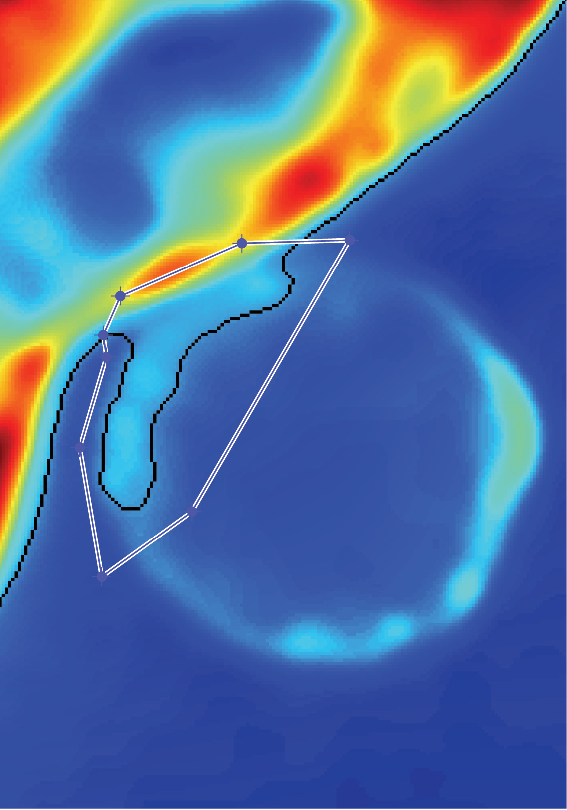
\includegraphics[width=0.249\textwidth]{mask-e.pdf}}
\subfloat[\label{mask-e} Result of deletion]{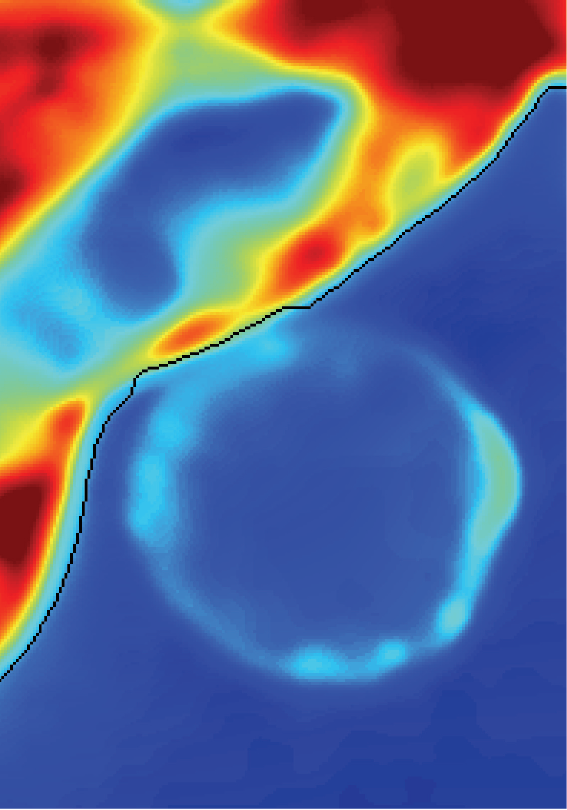
\includegraphics[width=0.249\textwidth]{mask-f.pdf}}
\end{figure}

%  %%
%  
%  \begin{figure}
%  \caption[ISAT]{\label{fig: ISATComp} \emph{ISAT}. The automatic segmentation in (a,c,e,g) are done by manually chosing a global threshold followed by contour smoothing and hole filling. Their results are weak for skeletonization compared to ISAT results. In (a) several dendrites (left, bottom) are shortened, and in (e), the lower right branch is missing and the branching point is in wrong poision (shown in white polygons). The skeletonization uses Bai's method (see below).}
%  \subfloat[No ISAT]{\includegraphics[angle=270,width=0.25\textwidth]{noISATResNeuronPsd.pdf}}
%  % \subfloat[No ISAT]{\includegraphics[angle=270,width=0.25\textwidth]{noISATResNeuron.pdf}}
%  % Psd: photoshoped.
%  \subfloat[ISAT]{\includegraphics[angle=270,width=0.25\textwidth]{ISATResNeuron.pdf}}
%  \subfloat[No ISAT mask]{\includegraphics[angle=270,width=0.25\textwidth]{noISATBwNeuron.pdf}}
%  \subfloat[ISAT mask]{\includegraphics[angle=270,width=0.25\textwidth]{ISATBwNeuron.pdf}}\\
%  \subfloat[No ISAT]{\includegraphics[width=0.25\textwidth]{noISATResPollenPsd.pdf}}
%  \subfloat[ISAT]{\includegraphics[width=0.25\textwidth]{ISATResPollen.pdf}}
%  \subfloat[No ISAT mask]{\includegraphics[width=0.25\textwidth]{noISATBwPollen.pdf}}
%  \subfloat[ISAT mask]{\includegraphics[width=0.25\textwidth]{ISATBwPollen.pdf}}
%  \end{figure}
%  
%  \subsection{Hints for manual operations}
%  
%  \subsubsection{AI-first principle}
%  
%  Try to use \emph{add with AI} or \emph{delete with AI} whenever possible. This could reduce subjectivity, manual error and operation labor extensively, although sometimes the ROI by AI is rougher than the manual ROI especially when SNR is low. There is a case that the connection is broken due to the uneven fluorescence labeling or loss of focus because cell goes beyond the focus plane. The dark part makes the AI ROI addition failure. In this case, the user could first add the dark part manually at first, and then use AI ROI to add the rest brighit part.
%  
%  The global threshold could be adjusted at first at steps of 20 or 30, get a coarse range, and then try to tune the threshold in the range.
%  
%  The neuron image segmentation requires a lot more efforts than pollen images, because the low SNR makes the intelligent addition or deletion weak (in this case, the region by AI is very rough; then the manual operated region, which is a polygonal contour, looks smoother than the region by AI), and the more annoying is that the branches from neuron soma touch or cross each other from time to time. When the touching occurs, the user need to distinguish which belongs to which. A very useful experience for this is that, the belongings could be judged based on the elongation angle. Usually the branch would take a turn in a range of +/- 60 degrees, so if there is an turn angle larger than 90, you may need to try assign in an alternative way.
%  
%  % \todo \textbf{Figure?}
%  
%  %%
%  % \begin{figure}
%  % \caption{\label{Figure: preprocRes} \emph{Preprocessing result image}.} \includegraphics[width=0.98\textwidth]{neuronPreproc-eps.pdf}
%  % \end{figure}
%  
%  \section{Cell body Masking}
%  
%  The position of the cell body, such as pollen grain and neuron soma, is also needed to extract meaningful morphological features. Yet, automatically recognizing the cell body automatically is difficult, as it is difficult to distinguish from a swollen tip that is present in many non-wildtype pollen. The masking of cell body is thus performed in a similar semi-automated manner as manual refinement of the segmentation based on RRs, except for that the initial segmentation is done by setting a higher global threshold or manually inputing an RR.
%  
%  %%%%%%%%%%%%%%
%  
%  % \chapter{Branching based features}
%  % \label{chap:branFeat}
%  
%  % \section{Morphological and textual features}
%  
%  % OWEN: Describe how you extract the skeleton and how you retrieve
%  % features from the skeleton.
%  
%  \section{Skeletonization}
%  
%  We used Bai's method \cite{Bai2007Skeleton} for skeletonization due to the robustness against small sharp edges on the segmentation of the underlying Discrete Contour Evolution (DCE) algorithm. As the number of branches in pollen tubes will always be below 5, we specified 13 as the maximum number of in the polygon similification by DCE.
%  
%  %In the cases that the magnification of
%  %microscopy is low and hence the pollen tubes are thin, image thinning with Matlab's ready-to-use functions is faster. If the branch numbers are larger than 5, image thinning method is also preferable to Bai's.
%  
%  For further processing, the resulting skeleton may not contain more than three mutual nieghbours in the 8-neighborhood of any pixels. Correspondingly, we eliminated such redunant pixels without affecting the connectedness or topology of the skeleton.
%  
%  \subsection{Parsi-skeletionization}
%  
%  The aim of Parsimoniusly skeletionization is to assure each foreground pixel have no more than 3 8-way neighours, e.g. pixels of on the center part have 2 8-neighbours, while pixels at branching junction have 3 8-neighbours.
%  
%  % % TODO: an image explaining 4-way and 8-way neighbours is needed?
%  
%  % For example, if a pixel has close 4-neighbours, where they form a L-shape\\
%  % \begin{verbatim}
%  % @@@
%  % @
%  % @
%  % \end{verbatim}
%  % will be reduced to\\
%  % \begin{verbatim}
%  %  @@
%  % @
%  % @
%  % \end{verbatim}
%  % While a straight line
%  % \begin{verbatim}
%  % @@@@@@@
%  % \end{verbatim}
%  % 
%  % \noindent will be kept.
%  
%  % \todo{Ren-shape?}
%  
%  The whole workflow of branMorph is summarized as in \figRef{fig: branMorphFlow}.
%  
%  \begin{figure}
%  \caption[Workflow of branMorph]{\label{fig: branMorphFlow} \emph{Workflow of branMorph}. The four intermediate outputs: intensity image, cell mask, cell body mask and skeleton image are represented in black ellipses. These outputs are used to perform feature extraction later on. Adj.Mat. is short for adjacency matrix.}
%  \includegraphics[width=0.9999\textwidth]{branMorphFlow.pdf}
%  \end{figure}
%  
%  \section{Feature extraction}
%  
%  When having the four intermediate results shown in \figRef{fig: branMorphFlow} at hand, the features could be extracted easily.
%  
%  \subsection{Tracing}
%  
%  To identify lengths parameters of the pollen tube and braches, the skeleton needs to represented as a graph, which we perform in a \emph{tracing} step. Tracing strarts with identifying all \emph{end points} (skeleton points with only 1 8-neighbor) as well as all \emph{junction points} (skeleton points with 3 8-neighbors). The set of all end points and junction points constitutes the set of all vertices in the graph representation. The distances between connected vertices are then obtained by simply tracing the connecting edges of the skeleton, yielding an adjacency matrix $A$.
%  
%  \subsection{Branch Length Features}
%  
%  We used Floyd's algorithm to transform the adjacency matrix $A$ into a distance matrix $D$. Setting the nearest end point to the pollen grain mask as a starting point $a$ (See Figure~\ref{Figure: branchDemo}), the furthest point to the starting point is found in $D$ denoted as $b$. The skeleton part connecting $a$ and $b$ is the longest branch that we also refer to as the \emph{backbone}. In a similar way, we can get the longest sub-branch on the longest branch. Both the length of the backbone and the length of the longest sub-branch are computed as features representing pollen tube morphology. In addition, the relative branching position as the fraction between \emph{(i)} the distance from the pollen grain to the branching point of the longest sub-branch and \emph{(ii)} the length of the backbone is also recorded.
%  
%  % \textbf{TODO:} \emph{MAKE A FIGURE FOR THIS!}
%  
%  % \begin{figure}
%  % \caption{\label{Figure: branchDemo} \emph{An example showing the features along the skeleton}. $a$: Starting point on the backbone. $b$: End point on the backbone. Blue Circle: pollen grain. Magenta Circle: branch tip. Cyan Circle: significant swollen bubbles. Thick white lines: the skeleton. Thin white tube is the longest backbone with estimated width.} \includegraphics[width=\textwidth]{branchDemo-eps.pdf}
%  % \end{figure}
%  
%  \begin{figure}
%  \caption[Artificial example image showing the features along the skeleton]{\label{Figure: branchDemo} \emph{Artificial example image showing the features along the skeleton}.$a \to b$ is the longest backbone, and $h \to c$ is the longest child branch on $a \to b$. $d \to e$ and $f \to g$ are two other first level branches which start out from pollen grain. Blue Circle: pollen grain. Magenta Circle: branch tip. Red Circle: significant swollen bubbles. Thick white lines: the skeleton. Thin white tube is the longest backbone with estimated width.}
%  % \caption{\label{Figure: artImg} \emph{Artificial image}.}
%  %\subfloat{\includegraphics[width=0.42\textwidth]{branchDemo-eps.pdf}} ~\
%  %\subfloat{\includegraphics[width=0.53\textwidth]{057.pdf}}
%  
%  %\begin{figure}
%  %\caption{\label{Figure: artImg} \emph{Artificial image}.}
%  \includegraphics[width=0.98\textwidth]{branMorphDemoPlot.pdf}  
%  %\end{figure}
%  
%  \end{figure}
%  
%  
%  \subsection{Width and Diameter Features}
%  
%  The pollen tube width and tip width are very important descriptors for mutants. To assess the widths, we used the distance transform of segmentation, traced along the path where the \emph{backbone} resides, and consequently produced a backbone profile. After smoothing, the median of all minima on the profile is used as an estimator for the tube width, and the significant maxima are recorded as swollen bubbles. The tip width takes the value of the first maxima of non-smoothed profile in the direction from tip to pollen grain. Therefore, we have backbone width, backbone tip width, bubbles' relative position and bubbles' radia.
%  
%  
%  \subsection{Waviness}
%  
%  We used a matlab script \footnote{\url{http://www.mathworks.com/matlabcentral/fileexchange/30793}, accesed on Mar 26th, 2012} to gain an extensively smoothed backbone. The script used Gaussian Weighted Least Squares to fit the original contour and got a smoothed line, then projected the original curve points onto the line to gain a smoothed curve with same number of points. Using a smoothing radius of about 200 achieved a center line we expected, as in \figRef{Figure: smoothContourEdgePad} (upper). When using the radius $r = 301$, the smoothing didn't improve much while resulted in the longer untouched edges. Therefore we chose $r = 201$. The original script uses a Copy-Original-At-Edge (COAE) strategy, to keep the points on both ends of the curve as they are without smoothing and projection. We found it's fully possible to pad the ends by mirroring the edge points, so that the curve smoothing is totally achieved without any intact corner (see \figRef{Figure: smoothContourEdgePad}, lower).
%  
%  \begin{figure}
%  \caption[Contour smoothing using different radius]{\label{Figure: smoothContourEdgePad} \emph{Contour smoothing using different radius}. \textbf{Upper}: Contour smoothing without edge padding. \textbf{Lower}: Coutour smoothing with edge mirror-padded. The larger the radius is, the more the smoothed contour from the start point (lower-left at both figures) keep unchanged since the original script uses a Copy-Original-At-Edge (COAE) strategy. The black boxes in both images show the major difference, that the centerline is well determined with edge padding in \textbf{(b)}, while not without edge padding \textbf{(a)}. The x-axis and y-axis are not on the same scale because both figures are zoom-ins taken without keeping aspect-ratio in order to exagerate the deviations.}
%  
%  \subfloat[Without edge padding]{\includegraphics[width=\textwidth]{smoothContourDemo2.pdf}}\\
%  \subfloat[With edge padding]{\includegraphics[width=\textwidth]{smoothContourEdgePad2.pdf}}
%  
%  \end{figure}
%  
%  We propose here two features related to the wavy type: \emph{wavy coefficient} and \emph{wavy number}. \emph{wavy coefficient}, or \emph{wavyCoef}, is defined as $\sum{d}/l$, where $d$ is the absolute deviations of the backbone curve from its smoothed center line, and $l$ is the backbone length. We used the wavelet-based automaton peak picking method (here denoted as \emph{wavePick}) from \Textcite{Li2011Circulation} to pick significant peaks on the absolute deviations (see \figRef{fig: wavePick}). The peak number is taken as the second feature \emph{wavy number}.
%  
%  % $\vec{d}$
%  
%  \begin{figure}
%  \caption[WavePick and wavy picked]{\label{fig: wavePick} \emph{WavePick and waviness peaks picked}.}
%  \subfloat[Picked peaks]{\includegraphics[width=\textwidth]{wavePick2.pdf}}\\
%  \subfloat[Corresponding waviness recognized]{\includegraphics[width=\textwidth]{wavyDemo.pdf}}
%  \end{figure}
%  
%  \subsection{Features summary}
%  
%  Together with the area of pollen grain mask, we obtain a list of 12 features listed in Table \ref{tab:features}.
%  
%  %	\begin{table}
%  %	  \centering
%  %	\begin{tabular}{|l|}
%  %	\hline Features\\ \hline \emph{Pollen area}\\ \emph{Backbone length}\\ \emph{Backbone child number}\\ \emph{Number of branches starting from pollen grain}\\ \emph{Relative branching position}\\ \emph{Secondary backbone length}\\ \emph{Backbone width}\\ \emph{Backbone tip width}\\ \emph{Secondary backbone width}\\ \emph{Secondary backbone tip width}\\ \emph{Bubble number}\\ \emph{Radium of largest bubble}\\ \emph{Ratio of backbone tip width and backbone width}\\ \emph{The standard deviation of intensities along backbone skeleton}\\ \emph{Ratio of pollen tube average intensity and pollen grain average intensity}\\ \emph{Wavy coefficient}\\ \emph{Wavy number}\\ \hline
%  %	\end{tabular}
%  %	  \caption{List of morphometric features}
%  %	  \label{tab:features}
%  %	\end{table}
%  
%  \begin{table}
%  \caption[List of morphometric features]{\emph{List of morphometric features}. The third column gives the calculated feature values of the example image in \figRef{Figure: branchDemo}.}
%  \label{tab:features}
%  {\scriptsize \tt
%  \begin{tabular}{ccc}
%  \hline
%  Features & Abbreviations & Example values\\\hline
%  %psArea, bbLen, bbChildNum, flBrNum, sbPos, ...
%  %    sbLen, bbWidth, bbTipWidth, sbWidth, sbTipWidth, ...
%  %    bubbleNum, lbRad, widthRatio, bbIntStd, avgIntRatio,wavyCoef,wavyNum
%  \emph{Pollen grain area}		&		psArea	&	9519\\\hline
%  \emph{Longest backbone length}	&		bbLen	&	607\\\hline
%  \emph{Longest backbone child number}	&	bbChildNum	&	2\\\hline
%  \emph{Number of branches starting from pollen grain}	&	flBrNum	&	3\\\hline
%  \emph{Relative branching position}		&		sbPos	&	0.2\\\hline
%  \emph{Secondary backbone length}		&		sbLen	&	304.4\\\hline
%  \emph{Longest backbone width}					&		bbWidth	&	16.4\\\hline
%  \emph{Longest backbone tip width}				&		bbTipWidth	&	44.0\\\hline
%  \emph{Secondary backbone width}			&		sbWidth	&	11.1\\\hline
%  \emph{Secondary backbone tip width}		&		sbTipWidth	&	19.9\\\hline
%  \emph{Total bubble number}		&	bubbleNum	&	2\\\hline
%  \emph{Radius of largest bubble}		&	lbRad	&	43.6\\\hline
%  \emph{Ratio of backbone tip width and backbone width}	&	widthRatio	&	2.7\\\hline
%  \emph{The standard deviation of intensities along backbone skeleton}		&	bbIntStd	&	0\\\hline
%  \emph{Ratio of average intensity between tube and grain}		&	avgIntRatio	&	1.0\\\hline
%  \emph{Wavyness coefficient}		&	wavyCoef	&	4.6\\\hline
%  \emph{Number of waves}			&	wavyNum	&	9\\\hline
%  \end{tabular}
%  }
%  \end{table}
%  
%  \section{Time consumption}
%  
%  Using the method proposed here, we can obtain tube lengths and other key morphometric features of pollen tubes in a highly reproducible manner within few minutes (the original image is 4080 pixels by 3072 pixels, and a crop-out of it is about 1000 pixels by 1000 pixels), thus making it suitable for studies involving in the order of several dozens of images.
%  
%  
%  % \chapter{Results}
%  
%  \section{Applications in classifying pollen tube images}
%  \label{sec: results}
%  
%  %%%%%%%%%
%  %	\section{Results}
%  %	
%  %	\subsection{Comparisons}
%  %	
%  %	We used our method to decompose the morphorlogical features of two data sets. One is organized in groups of distinct morphologies manually by pollen tube researchers, who summarized about 6 typical morphologies for the tobacco pollen tubes - Balloon-tip, Branching, Swollen-in-the-middle, Thin-tube, Wavy-tube, and Wildtype. \textbf{TODO??? 6 typical pollen image gallery.}
%  %	
%  %	The other data set is categorized into 4 groups according to the introduced genges by transfection/transformation?? as well as wildtype. They are - G145+G16, G16, W42, W32, and W32 is the wildtype.
%  %	
%  %	??? The G16's causing was validated in the research \cite{Kaothien2005Kinase}. We found no distinct separation between G145+G16 and G16 in the PCA of 4 groups. TODO: How about the PCA of only G145+G16?
%  %	
%  %	We used our method to get the skeleton features and showed them in the plot with the first two main components as x and y coordinates after Principal Component Analysis. For comparison, we also extracted all the murpy features and did PCA plots too. The codes used to generate murpy features were grabbed from \url{http://lanec1web1.compbio.cs.cmu.edu/release/SLIC_v3_0.tgz} on Mar 2012, and we turned on all features ('img', 'hul', 'edg', 'mor', 'zer', 'har', 'wav', 'skl', 'nof') the codes could get.
%  %	
%  %	As we can see, the skeleton features could distinguish the types in the first dataset. And for the second data set, G145+G16 distribute similarly with G16, which suggests the G145 has no effect providing G16 is in effect.
%  %	
%  %	\includegraphics[width=\textwidth]{ourTyp-eps.pdf}
%  %	
%  %	\includegraphics[width=\textwidth]{murphTyp-eps.pdf}
%  %	
%  %	\includegraphics[width=\textwidth]{ourGroup-eps.pdf}
%  %	
%  %	\includegraphics[width=\textwidth]{murphGroup-eps.pdf}
%  %	
%  %	The murpy features in total can not tell apart all the groups, which is not surprising as the murph features are purposed to describe the distribution of protein components in a cell, while our data focuses on the shape differences, with only one connected component in each image. Therefore, the SLF1 features, which describes the number of components, the euler number, etc, can help with nothing here. Considering these, we used feature selection method based on Random Forest (\url{code.google.com/p/randomforest-matlab/}) to check what features in murphy features helped in distinguish between groups.
%  
%  %%%%%%%%%%%%%%%%%%
%  
%  % \subsection{Distinguish on simulated image data}
%  
%  \subsection{Distinguish on data grouped by morphologies}
%  \label{subsec: morphGroup}
%  
%  % We used our method to extract features described above on the human annotated morphological dataset (as the dataset 1 in the Materiel section).
%  % The dataset is in groups of distinct morphologies organized and annotated manually by pollen tube researchers, who summarized about 6 typical morphologies for the tobacco pollen tubes regarding the outline shape - Balloon-tip, Branching,
%  % Swollen-in-the-middle, Thin-tube, Wavy-tube, and Wildtype. The data sets are descripted in detail in Supplimentary part.
%  
%  A set of microscopic images displaying tobacco pollen tube growth under different constructs were classified into phenotype groups by a human expert. The annotation assigns each image into one out of six pollen tube phenotype groups. Representative images for each of the six phenotype groups \emph{balloon tip}, \emph{branching}, \emph{swollen}, \emph{thin}, \emph{wavy}, and \emph{wildtype} are displayed in Supplementary figures, and the complete data set is displayed in Supplement tables. This partitioning into phenotype groups served as a reference ``ground truth'' partitioning that we aimed to reconstruct using supervised classifiers on the image features listed in Table \ref{tab:features}. We will name these features in the following sections as \emph{skeleton based features} since the calculation starts from the process of image skeletonization. We compared the classification performance obtained from our features to the performance obtained from the Murphy's feature set provided in the \emph{SLIC} library (\footnote{\url{http://lanec1web1.compbio.cs.cmu.edu/release/SLIC_v3_0.tgz}, accessed on Mar 2012.}), implementing the sub-cellular location features described in \parencite{Boland1998Automated}. For our study, we utilized the complete feature set provided in the \emph{SLIC} library.
%  
%  \figRef{Figure: pca-a} indicates the adequacy of our features to distinguish the different phenotypes observable in our data set based on the first two principal components. To further support this on a more quantitative basis, we examined the cross-validation performance of a random forest classifier. We used 100,000 trees and Leave-One-Out-Cross-Validation (LOOCV) strategy to train and validate the classifier. To determine the optimal number $P$ of predictors at each node, we evaluated a range of values experimentally, yielding an error rate of 0.22 for the optimal choice. The variables \emph{wavyNum}, \emph{bbTipWidth}, \emph{bbIntStd}, \emph{wavyCoef} are most relevant for distinguishing the different phenotypes, as indicated by their Gini indices of $1.40$, $1.18$, $1.17$, and $1.12$ respectively. In comparison, the $130$ sub-cellular location features by Murphy yield an error rate of $0.56$. The features \emph{obj\_skel\_len}, \emph{obj\_skel\_branch\_per\_len}, \emph{entropy}, \emph{W\_h6} ranked highest with Gini index of $0.98$, $0.94$, $0.8$, and $0.41$, respectively.
%  
%  We also investigated the classification errors for systematic errors by studying the confusion matrices as shown in \tabRef{Table: confmat1}.
%  
%  % The \emph{normalized} here indicates that the numbers in the original matrix are divided by the true data number per class. The actual confusion matrices are given in \tabRef{Table: confmat1}.
%  
%  % And for the second data set, G145+G16 distribute similarly with G16, which suggests two possibilities: 1, the G145+G16 may be similar to G16 and no differece is between. 2, the features we used altogether disguise the difference.
%  
%  % The Murphy features have little help in such kind of job, although they are good at distinguish the protein subcellular distributions. It is not surprising as the murph features are purposed to describe the distribution of protein components in a cell, while our data focuses on the shape differences, with only one connected component in each image. Therefore, the SLF1 features, which describes the number of components, the euler number, etc, can help with nothing here.
%  
%  % Considering these, we used feature selection method based on Random Fores to check what features in murphy features helped in distinguish between groups.
%  
%  % As we can see, the skeleton features could easily distinguish the morphological types in the dataset. And for the second data set, G145+G16 distribute similarly with G16, which suggests two possibilities: 1, the G145+G16 may be similar to G16 and no differece is between. 2, the features we used altogether disguise the difference.
%  
%  % In order to clarify the second possibility, we assumed it being true. We grabbed only the G145+G16 and G16 and did classification on the two groups with random forest \footnote{\url{code.google.com/p/randomforest-matlab/}} followed by performing feature selection. We used 10000 trees and One-out-of-Bag (OOB) Strategy to train and validate the classifier. In each OOB iteration, we ranked the first 3 most important features distinguishing the two groups, and gave each hit features a vote. The total sample number of the two groups is 34, and the most important features selected is: bbWidth - 34 votes, bbTipWidth - 34, avgIntRatio - 34. And the average error rate: 0.176471.
%  
%  % \textbf{TODO}: a group t-test or ANOVA is needed here. Extract only the 3 feature values and compare the difference between G145+G16 and G16.
%  
%  % The result met the expectation of the researcher since they thought the difference between G16 and G145+G16 resides on the backbone width and tip width.
%  
%  % \subsection{Distinguish on gene-classified data}
%  
%  % \begin{figure}
%  % \caption{\label{Figure: pca} \emph{PCA result on all features}.}
%  
%  % The other data set is categorized into 3 groups according to the introduced genges by microprojectile bombardment \parencite{Twell: 1989} in addition to the wildtype, labeled as - G16, W42, W32, and W32 is the wildtype.
%  
%  % The murpy features in total can not tell apart all the groups, which is not surprising as the murph features are purposed to describe the distribution of protein components in a cell, while our data focuses on the shape differences, with only one connected component in each image. Therefore, the SLF1 features, which describes the number of components, the euler number, etc, can help with nothing here. Considering these, we used feature selection method based on Random Fores to check what features in murphy features helped in distinguish between groups.
%  
%  % We also tried random forest on only the G145+G16 and G16 data. The most important features: W\_v7 - 34 votes, W\_d9 - 34, correlation - 33. The average error rate: 0.147059.
%  
%  \begin{table}
%  \caption[Confusion Matrices of features in machine learning]{\label{Table: confmat1} \emph{Confusion Matrices of features in machine learning}. (a-b): Confusion matricies on data grouped by morphology; (c-d): Confusion matrices on data grouped by genes. Rows show the actual class labels, and columns show the predicted labels by machine learning. The larger the numbers in the diagonal are, the better is the feature set's performance. In (a) and (b), in the row of \emph{swollen}, the only non-zero number is 1, and it indicates that this \emph{swollen} sample is predicted wrongly as \emph{wildtype}. The failure to classify the \emph{swollen} type in the third row  is due to the small sample size. The skeleton features also have difficulty in telling \emph{thin} from \emph{wildtype} for the two groups are mostly similar. See Supplement for detail. In (c) and (d), the skeleton features distinguish all three groups well, while \emph{SLIC} features are weak to distinguish G16 from W32.}
%  
%  {\scriptsize \tt
%  \begin{tabular}{ccccccc}
%  %\hline
%  \multicolumn{7}{l}{(a) Using skeleton based features}\\\hline
%  \backslashbox{True}{Predicted}		&	Balloon	& Branch 	&	Swollen & Thin & Wavy & Wildtype \\\hline
%  Balloon		&	2		&   0     	&	0		&  0   & 0    &	0\\\hline
%  Branch		&	0		&   6     	&	0		&  0   & 0    &	0\\\hline
%  Swollen		&	0		&   0     	&	0		&  0   & 0    &	1\\\hline
%  Thin		&	0		&   0     	&	0		&  1   & 0    &	2\\\hline
%  Wavy		&	0		&   0     	&	0		&  0   & 2    &	1\\\hline
%  Wildtype	&	0		&   0     	&	0		&  1   & 1    &	1\\\hline
%  \end{tabular}\vspace{0.2in}
%  
%  \begin{tabular}{ccccccc}
%  %\hline
%  \multicolumn{7}{l}{(b) Using \emph{SLIC} features}\\\hline
%  \backslashbox{True}{Predicted}		&	Balloon	& Branch 	&	Swollen & Thin & Wavy & Wildtype \\\hline
%  Balloon		&	0		&   2     	&	0		&  0   & 0    &	0\\\hline
%  Branch		&	0		&   6     	&	0		&  0   & 0    &	0\\\hline
%  Swollen		&	0		&   1     	&	0		&  0   & 0    &	0\\\hline
%  Thin		&	0		&   0     	&	0		&  2   & 0    &	1\\\hline
%  Wavy		&	0		&   0     	&	1		&  0   & 0    &	2\\\hline
%  Wildtype	&	0		&   1     	&	0		&  0   & 2    &	0\\\hline
%  \end{tabular}\vspace{0.2in}
%  
%  \begin{tabular}{cccc}
%  % \hline
%  \multicolumn{4}{l}{(c) Using skeleton based features}\\\hline
%  \backslashbox{True}{Predicted}	&	G16		& W32 		&	W42\\\hline
%  G16		&	10		&   1     	&	3	\\\hline
%  W32		&	1		&   16     	&	0	\\\hline
%  W42		&	2		&   0     	&	0	\\\hline
%  \end{tabular}
%  \begin{tabular}{cccc}
%  % \hline
%  \multicolumn{4}{l}{(d) Using \emph{SLIC} features}\\\hline
%  \backslashbox{True}{Predicted}	&	G16		& W32 		&	W42\\\hline
%  G16		&	6		&   7     	&	1	\\\hline
%  W32		&	4		&   12     	&	1	\\\hline
%  W42		&	0		&   0     	&	12	\\\hline
%  \end{tabular}
%  }
%  
%  \end{table}
%  
%  \newpage
%  
%  \begin{figure}
%  \caption[Distinguishing pollen tube data with features]{\label{fig: realPca} \emph{Distinguishing pollen tube data with features}. \protect\subref{Figure: pca-a} and \protect\subref{Figure: pca-b}: morphology-grouped data. \protect\subref{Figure: pca-c} and \protect\subref{Figure: pca-d}: gene-grouped data. The blue lines represent the feature vectors, and we could easily infer the feature contribution to the first two principal components from its projections on each axis. In \protect\subref{Figure: pca-a}, we could see \emph{bubbleNum}, \emph{widthRatio}, \emph{sbTipWidth}, \emph{bbWidth} and \emph{wavyNum} contribute most to the two principal components. And \emph{flBrNum} is helpless here since all pollen tubes have only 1 first level branch (see supplementary). In \protect\subref{Figure: pca-c}, the three groups different in gene constructs have distinct distribution in the PCA plane axised by the first two principal components. We also can infer here that the \emph{bbTipWidth}, \emph{widthRatio}, \emph{avgIntRatio} and \emph{psArea} contribute most in distinguishing between these groups, however the \emph{wavyCoef} and \emph{bbIntStd}, which contribute most to the second principal component, helps little in telling the 3 groups apart. In \protect\subref{Figure: pca-b} and \protect\subref{Figure: pca-d}, all variable labels are removed for clarity, and the plot with variable labels could be found in supplementary.}
%  % \subfloat[\label{Figure: pca-a} Our features on data set 1]{\includegraphics[width=0.48\textwidth]{ourTyp-eps.pdf}}
%  % \subfloat[\label{Figure: pca-b} Murphy features on dataset 1]{\includegraphics[width=0.48\textwidth]{murphTyp-eps.pdf}}\\
%  % \subfloat[\label{Figure: pca-c} Our features on dataset 2]{\includegraphics[width=0.48\textwidth]{ourGroup2.pdf}}
%  % \subfloat[\label{Figure: pca-d} Murphy features on dataset 2]{\includegraphics[width=0.48\textwidth]{murphGroup2.pdf}}
%  
%  \subfloat[\label{Figure: pca-a} Features from Table \ref{tab:features}]{\includegraphics[width=0.98\textwidth]{ourTypPca16pt.pdf}}\\
%  % ourMorphPca.pdf
%  % \subfloat[\label{Figure: pca-b} \emph{SLIC} features]{\includegraphics[width=0.98\textwidth]{murphTypPcaNolabel.pdf}}
%  \subfloat[\label{Figure: pca-b} \emph{SLIC} features]{\includegraphics[width=0.98\textwidth]{murphTypPca.pdf}}
%  % \subfloat[\label{Figure: conf-a} Confusion Matrix of random forest classifier for features from Table \ref{tab:features}]{\includegraphics[width=0.48\textwidth]{confmatTypSkel.pdf}}
%  % \subfloat[\label{Figure: conf-b} Confusion Matrix of random forest classifier for SLIC features]{\includegraphics[width=0.48\textwidth]{confmatTypMurph.pdf}}\\
%  \end{figure}
%  
%  \begin{figure}
%  \ContinuedFloat
%  \caption[Distinguishing pollen tube data with features]{\emph{Distinguishing pollen tube data with features}, cont.}
%  % \caption{\emph{Distinguish on images grouped by genes}. The three groups different in gene constructs have distinct distribution in the PCA plane of first two principal components. We also can infer here that the \emph{bbTipWidth}, \emph{widthRatio}, \emph{avgIntRatio} and \emph{psArea} contribute most in distinguishing between these groups, however the \emph{wavyCoef} and \emph{bbIntStd}, which contribute most to the second principal component, helps little in telling the 3 groups apart. In \subref{Figure: pca-d}, all variable labels are removed for clarity, and the plot with variable labels could be found in supplementary.}
%  \subfloat[\label{Figure: pca-c}Features from Table \ref{tab:features}]{\includegraphics[width=0.98\textwidth]{ourGroupPca16pt.pdf}}\\
%  % ourGenesPca.pdf
%  % \subfloat[\label{Figure: pca-d} \emph{SLIC} features]{\includegraphics[width=0.98\textwidth]{murphGroupPcaNolabel.pdf}}
%  \subfloat[\label{Figure: pca-d} \emph{SLIC} features]{\includegraphics[width=0.98\textwidth]{murphGroupPca.pdf}}
%  % \subfloat[\label{Figure: conf-a} Confusion Matrix of random forest classifier for features from Table \ref{tab:features}]{\includegraphics[width=0.48\textwidth]{confmatGroupSkel.pdf}}
%  % \subfloat[\label{Figure: conf-b} Confusion Matrix of random forest classifier for SLIC features]{\includegraphics[width=0.48\textwidth]{confmatGroupMurph.pdf}}\\
%  \end{figure}
%  
%  \subsection{Classification of simulated pollen tube images}
%  
%  The \emph{swollen} phenotype has only one data in our data set and therefore affects the classification accuracy when LOOCV strategy is used. However, the result that the groups are well separated in PCA plane as in \figRef{fig: realPca} shows that the skeleton-based features are sufficiently powerful in classifying the morphological groups. To further prove it, We simulated a set of pollen tube images and tested our method on the data set. The results shown in \figRef{fig: simuRes} and \tabRef{tab: simuRes} demonstrate the classification power of our skeleton-based features.
%  
%  \begin{figure}
%  \caption{\label{fig: simuRes} \emph{Simulated pollen tube images on PCA planes}.}
%  \subfloat[Skeleton features]{\includegraphics[width=0.98\textwidth]{simuPollenPcaSidebar.pdf}}\\
%  \subfloat[\emph{SLIC} features (variable labels removed for clarity)]{\includegraphics[width=0.98\textwidth]{murphSimuPca.pdf}}
%  \end{figure}
%  
%  
%  \begin{table}
%  \caption[Classification results of simulated pollen tube images]{\label{tab: simuRes} \emph{Classification results of simulated pollen tube images}. Imbalanced training data with 10 training samples for wildtype and 3 each for all other phenotypes \textbf{(c)} have minor impact on the classifier performance compared to balanced training data \textbf{(a)}, where all classes have 5 training and testing samples. In comparison, SLIC features perform poorly even on balanced training data \textbf{(b)}. Performance was measured using leave-one-out cross validation.}
%  {\scriptsize \tt
%  
%  %\subfloat[Skeleton features]{
%  \begin{tabular}{ccccccc}
%  %\hline
%  \multicolumn{7}{l}{(a) Using skeleton based features}\\\hline
%  \backslashbox{True}{Predicted}		&	Balloon	& Branch 	&	Swollen & Thin & Wavy & Wildtype \\\hline
%  Balloon		&	5	&   0  &	0	&  0   & 0    &	0\\\hline
%  Branch		&	0	&   5  &	0	&  0   & 0    &	0\\\hline
%  Swollen		&	0	&   0  &	5	&  0   & 0    &	0\\\hline
%  Thin		&	0	&   0  &	0	&  5   & 0    &	0\\\hline
%  Wavy		&	0	&   0  &	0	&  0   & 4    &	1\\\hline
%  Wildtype	&	0	&   0  &	0	&  0   & 0    &	5\\\hline
%  \end{tabular}
%  %}
%  \vspace{0.2in}
%  
%  %\subfloat[\emph{SLIC} features]{
%  \begin{tabular}{ccccccc}
%  % \hline
%  \multicolumn{7}{l}{(b) Using \emph{SLIC} features}\\\hline
%  \backslashbox{True}{Predicted}		&	Balloon	& Branch 	&	Swollen & Thin & Wavy & Wildtype \\\hline
%  Balloon		&	3  &  0  &  1  &  0  &  0  &  1\\\hline
%  Branch		&	0  &  2  &  1  &  0  &  2  &  0\\\hline
%  Swollen		&	1  &  0  &  3  &  0  &  0  &  1\\\hline
%  Thin		&	0  &  0  &  0  &  5  &  0  &  0\\\hline
%  Wavy		&	0  &  2  &  0  &  0  &  3  &  0\\\hline
%  Wildtype	&	2  &  0  &  1  &  1  &  0  &  1\\\hline
%  \end{tabular}
%  %}
%  
%  \begin{tabular}{ccccccc}
%  % \hline
%  \multicolumn{7}{l}{(c) Imbalanced training data; skeleton based features}\\\hline
%  % \multicolumn{3}{l}{(a) Using skeleton based features}\\\hline
%  \backslashbox{True}{Predicted}	& Wildtype	&	Balloon	& Branch 	&	Swollen & Thin & Wavy \\\hline
%  Wildtype	&	10 &  0  &  0  &  0  &  0  &  0\\\hline
%  Balloon		&	0  &  2  &  0  &  1  &  0  &  0\\\hline
%  Branch		&	0  &  0  &  3  &  0  &  0  &  0\\\hline
%  Swollen		&	0  &  0  &  0  &  3  &  0  &  0\\\hline
%  Thin		&	0  &  0  &  0  &  0  &  3  &  0\\\hline
%  Wavy		&	2  &  0  &  0  &  0  &  0  &  1\\\hline
%  \end{tabular}
%  
%  
%  }
%  \end{table}
%  
%  To address the issue on how our method will perform when encountering imbalanced data set, we extended the first data set to 10 artificial wildtype pollen tube images, and reduced all other phentype classes to 3 artificial pollen tube images. The influence on classifier performance was evaluated using leave-one-out cross validation as shown in \tabRef{tab: simuRes}, demonstrating robustness against imbalanced training data.
%  
%  % To address the issue on how our method will perform when encountering imbalanced data set, we used 10 artificial wildtype pollen tube images and mixed 3 artificial pollen tube images from one 'mutant' group (e.g., \emph{balloon}, \emph{branch}, \emph{swollen}, \emph{thin} and \emph{wavy}) each time to check if our method could distinguish abnormal morphological phenotypes from amounts of data. \tabRef{tab: imbaTest} shows that our method is able to fullfill such tasks.
%  
%  % \begin{table}
%  % \caption{\color{red} \label{tab: imbaTest} \emph{Classification on imbalanced simulated pollen tube images}. All except \emph{wavy} phenotypes are well distinguished from \emph{wildtype} under imbalanced condition.}
%  % {\scriptsize \tt
%  % 
%  % \begin{tabular}{ccc}
%  % \hline
%  % % \multicolumn{3}{l}{(a) Using skeleton based features}\\\hline
%  % \backslashbox{True}{Predicted}		&	Wildtype	& Balloon \\\hline
%  % Wildtype	&	10	&   0 \\\hline
%  % Balloon		&	0	&   3 \\\hline
%  % \end{tabular}
%  % \begin{tabular}{ccc}
%  % \hline
%  % % \multicolumn{3}{l}{(a) Using skeleton based features}\\\hline
%  % \backslashbox{True}{Predicted}		&	Wildtype	& Branch \\\hline
%  % Wildtype	&	10	&   0 \\\hline
%  % Branch		&	0	&   3 \\\hline
%  % \end{tabular}\vspace{0.2in}
%  % 
%  % \begin{tabular}{ccc}
%  % \hline
%  % % \multicolumn{3}{l}{(a) Using skeleton based features}\\\hline
%  % \backslashbox{True}{Predicted}		&	Wildtype	& Swollen \\\hline
%  % Wildtype	&	10	&   0 \\\hline
%  % Swollen		&	0	&   3 \\\hline
%  % \end{tabular}
%  % \begin{tabular}{ccc}
%  % \hline
%  % % \multicolumn{3}{l}{(a) Using skeleton based features}\\\hline
%  % \backslashbox{True}{Predicted}		&	Wildtype	& Thin \\\hline
%  % Wildtype	&	10	&   0 \\\hline
%  % Thin		&	0	&   3 \\\hline
%  % \end{tabular}\vspace{0.2in}
%  % 
%  % \begin{tabular}{ccc}
%  % \hline
%  % % \multicolumn{3}{l}{(a) Using skeleton based features}\\\hline
%  % \backslashbox{True}{Predicted}		&	Wildtype	& Wavy \\\hline
%  % Wildtype	&	10	&   0 \\\hline
%  % Wavy		&	2	&   1 \\\hline
%  % \end{tabular}
%  % 
%  % }
%  % \end{table}
%  
%  \subsection{Classification of pollen tubes with different gene-constructs}
%  
%  In practical use, the image data are often grouped by gene-constructs instead of morphology, such as experiments to investigate how the over-expression of different genes could make change on the cell morphology, the image data in the experiments being grouped by genes but not the morphology \parencite{Kaothien2005Kinase, Zhang2008Pollen}.
%  
%  % are over-expressing LePRK-eGFP, and G16 are over-expressing KPP-eGFP
%  
%  To validate in such cases, We applied our method to a second data set, which is categorized into three groups according to the introduced genes by micro-projectile bombardment \parencite{Twell1989transient} in addition to the wildtype, labeled as G16, W42, and W32 \footnote{The gene names are to be published in another independent article focusing on experiment findings, so they are anonymized here in codes without confusing or misleading the methodology topic}. W32 are pollen tubes expressing GFP only, and W42 and G16 are over-expressing various pollen proteins fused with GFP. As we could see from \figRef{Figure: pca-c}, the skeleton features could tell apart the wildtype and the different gene constructs.
%  
%  We also tried the Murphy features, which in total can not tell apart all the groups, again (\figRef{Figure: pca-d} and \tabRef{Table: confmat1}).
%  
%  % We also evaluated the classification performance of a random forest
%  % classifier on the G145+G16 vs. G16 data, yielding an error rate of
%  % $.15$. The most important features turned out to be W\_v7,
%  % W\_d9, and correlation - 33.
%  
%  %	\section{Random forest}
%  %	
%  %	We used random forest to classify the datasets through the skeleton features and murphy features. The feature importances are calculated by Gini index.
%  %	
%  %	\subsection{Default settings}
%  %	
%  %	The random forest itself has a setting for training sample number, and I set it to be N-1 (N is the total number of obs) so it runs a leave-one-out cross validation (LOOCV) in the training phase. The error rate is estimated by the trained model, which means, the error rate is the mean of the Out-of-bag (oob) error rates of all the decision trees.  And I sorted the Gini index either. The result is:
%  %	
%  %	\begin{verbatim}
%  %	In train phase, average error rate: 0.329111
%  %	Error rates for classes:
%  %	Balloon    Branch    Swollen    Thin    Wavy    Wildtype
%  %	0.00035    1.66667e-05    NaN    0.6628    0.320317    NaN   
%  %	Sorted variables: widthRatio    wavyNum    bbTipWidth    wavyCoef.
%  %	Gini index: 1.21056    1.13977    1.04688    1.01785.
%  %	\end{verbatim}
%  %	
%  %	And I also tried the Leave-one-out cross-validation outside the frame of random forest. The error rates is the average of all the trials:
%  %	\begin{verbatim}
%  %	Predict phase: average error rate: 0.333333
%  %	\end{verbatim}
%  %	
%  %	All random forests used 10,000 trees.
%  %	One point is that, the error rate given at training phase is always changed at different runs, and the error rate of 0.333333 is always the same.
%  %	
%  %	\subsection{Find the optimal mtry}
%  %	
%  %	The optimal \emph{mtry} is to be found by trial runs. We ran random forest on the first dataset using $mtry=1\ldots20$. The number of features is 17, so the error rates of mtry larger than 17 are higher. Therefore, we try to find the optimal $mtry$ in the range of 1 to the number of features.
%  %	
%  %	The following runs are all using tree number of 100,000.
%  %	
%  %	\begin{verbatim}
%  %	
%  %	In train phase, average error rate: 0.496779. mtry=1.
%  %	In train phase, average error rate: 0.371454. mtry=2.
%  %	In train phase, average error rate: 0.331906. mtry=3.
%  %	In train phase, average error rate: 0.349484. mtry=4.
%  %	In train phase, average error rate: 0.338798. mtry=5.
%  %	In train phase, average error rate: 0.330423. mtry=6.
%  %	In train phase, average error rate: 0.299853. mtry=7.
%  %	In train phase, average error rate: 0.310069. mtry=8.
%  %	In train phase, average error rate: 0.313708. mtry=9.
%  %	In train phase, average error rate: 0.287941. mtry=10.
%  %	In train phase, average error rate: 0.266633. mtry=11.
%  %	In train phase, average error rate: 0.283562. mtry=12.
%  %	In train phase, average error rate: 0.257919. mtry=13.
%  %	In train phase, average error rate: 0.243671. mtry=14.
%  %	In train phase, average error rate: 0.226838. mtry=15.
%  %	In train phase, average error rate: 0.23548. mtry=16.
%  %	In train phase, average error rate: 0.232398. mtry=17.
%  %	In train phase, average error rate: 0.332477. mtry=18.
%  %	In train phase, average error rate: 0.332407. mtry=19.
%  %	In train phase, average error rate: 0.337222. mtry=20.
%  %	The smallest error rate is 0.226838, mtry=15
%  %	In train phase, average error rate: 0.223604
%  %	Error rates for classes: 
%  %	Balloon		Branch	Swollen		Thin	Wavy	Wildtype
%  %	0.00024	NaN	NaN	0.666967	NaN	0.34047	
%  %	Sorted variables: wavyNum	bbTipWidth	bbIntStd	wavyCoef.
%  %	Gini index: 1.40848	1.17983	1.1691	1.12212.
%  %	
%  %	Predict phase: average error rate: 0.333333
%  %	C =
%  %	     2     0     0     0     0     0
%  %	     0     6     0     0     0     0
%  %	     0     0     0     0     0     1
%  %	     0     0     0     1     0     2
%  %	     0     0     0     0     2     1
%  %	     0     0     0     1     1     1
%  %	\end{verbatim}
%  %	
%  %	As for the murphy features, the total murphy feature number is 130.
%  %	
%  %	\begin{verbatim}
%  %	The smallest error rate is 0.534878, mtry=129.
%  %	
%  %	In train phase, average error rate: 0.555738
%  %	Error rates for classes: 
%  %	Balloon		Branch		Swollen		Thin	Wavy	Wildtype
%  %	0.99999	0.000243667	NaN	0.334323	1	NaN	
%  %	Sorted variables: obj_skel_len	obj_skel_branch_per_len	entropy	W_h6.
%  %	Gini index: 0.983472	0.939755	0.799901	0.41082.
%  %	
%  %	Predict phase: average error rate: 0.555556
%  %	C =
%  %	     0     2     0     0     0     0
%  %	     0     6     0     0     0     0
%  %	     0     1     0     0     0     0
%  %	     0     0     0     2     0     1
%  %	     0     0     1     0     0     2
%  %	     0     1     0     0     2     0
%  %	\end{verbatim}
%  %	
%  %	As for the second data set,
%  %	
%  %	Use skeleton features,
%  %	\begin{verbatim}
%  %	The smallest error rate is 0.162501, mtry=46.
%  %	
%  %	In train phase, average error rate: 0.162996
%  %	Error rates for classes: 
%  %	G16	W32	W42	
%  %	0.28589	0.0588618	0.167142	
%  %	Sorted variables: widthRatio	bbTipWidth	avgIntRatio	psArea.
%  %	Gini index: 5.68333	5.56792	3.91448	3.71087.
%  %	
%  %	Predict phase: average error rate: 0.162791
%  %	Confusion matrix:
%  %	    10     1     3
%  %	     1    16     0
%  %	     2     0    10
%  %	\end{verbatim}
%  %	
%  %	Use murphy features,
%  %	\begin{verbatim}
%  %	The smallest error rate is 0.261215, mtry=130.
%  %	
%  %	In train phase, average error rate: 0.278966
%  %	Error rates for classes: 
%  %	G16			W32			W42
%  %	0.428407	0.352772	5.98831e-05	
%  %	Sorted variables: sum_entropy	correlation	W_v5	sum_of_squares.
%  %	Gini index: 4.67176	3.29051	3.20104	1.87217.
%  %	
%  %	Predict phase: average error rate: 0.302326
%  %	C =
%  %	     6     7     1
%  %	     4    12     1
%  %	     0     0    12
%  %	\end{verbatim}
%  %	
%  %	We also investigated into the structure of decision errors and the normalized confusion matrices are shown. The \emph{normalized} here indicates that the numbers in the original matrix are divided by the true data number per class.
%  
%  % \begin{figure}
%  % \caption{Confusion matrices.}
%  % 
%  % \subfloat[Skeleton features, morphological groups]{\includegraphics[width=0.48\textwidth]{confmatTypSkel.pdf}}
%  % %\subfloat[Murphy, data 1]{\includegraphics[width=0.48\textwidth]{murphyMtry.pdf}}\\
%  % \subfloat[\emph{SLIC}, morphological groups]{\includegraphics[width=0.48\textwidth]{confmatTypMurph.pdf}}\\
%  % \subfloat[Skeleton features, simulated data]{\includegraphics[width=0.48\textwidth]{simuPollenConf.pdf}}
%  % \subfloat[\emph{SLIC}, simulated data]{\includegraphics[width=0.48\textwidth]{murphSimuConfmat.pdf}}\\
%  % \subfloat[Skeleton features, gene constructs]{\includegraphics[width=0.48\textwidth]{confmatGroupSkel.pdf}}
%  % \subfloat[\emph{SLIC}, gene constructs]{\includegraphics[width=0.48\textwidth]{confmatGroupMurph.pdf}}\\
%  % \subfloat[Skeleton features, imbalanced data]{\includegraphics[width=0.48\textwidth]{imbaConf.pdf}}\\
%  % \end{figure}
%  
%  % \todo{A demo graph: lots of morph images -> feature matrix -> pca plane.}

